\immediate\write18{tex braids.dtx}
%\documentclass[border=10pt]{standalone}
\documentclass{article}
\usepackage{tikz}
\usepackage{braids}

\begin{document}

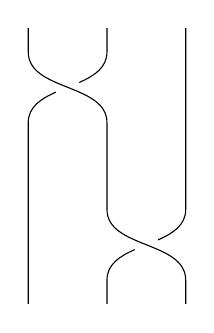
\begin{tikzpicture}
\braid a_1 1 a_2;
\end{tikzpicture}

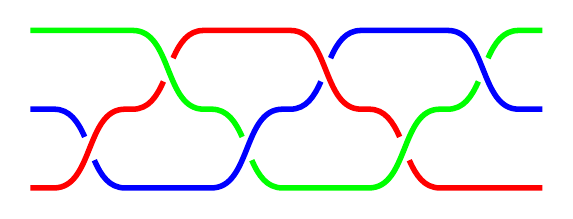
\begin{tikzpicture}
\braid[
  rotate=90,
  line width=2pt,
  style strands={1}{red},
  style strands={2}{blue},
  style strands={3}{green},
] a_1 a_2^{-1} a_1 a_2^{-1} a_1 a_2^{-1};
\end{tikzpicture}
%\end{document}

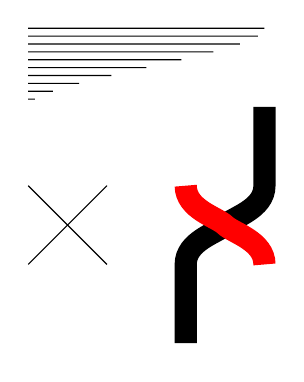
\begin{tikzpicture}
\begin{scope}[yshift=2cm]
\foreach \brtime in {0.1,0.2,...,1} {
\pgfpathcurvebetweentime{0}{\brtime}{\pgfpointxy{0}{\brtime}}{\pgfpointxy{0}{\brtime}}{\pgfpointxy{3}{\brtime}}{\pgfpointxy{3}{\brtime}}
}
\end{scope}

\pgfmathsetmacro{\bht}{0}
\draw (0,0) .. controls +(0,\bht) and +(0,-\bht) .. (1,1);
\draw (1,0) .. controls +(0,\bht) and +(0,-\bht) .. (0,1);
\begin{scope}[xshift=2cm]
\pgfmathsetmacro{\bht}{0.3}
\pgfmathsetmacro{\bdht}{0.1}
\draw[line width=8pt] (0,-1) -- (0,0) .. controls +(0,\bht) and +(-\bdht,-\bdht) .. (.5,.5) .. controls +(\bdht,\bdht) and +(0,-\bht) .. (1,1) -- +(0,1);
\draw[line width=8pt,red] (1,0) .. controls +(0,\bht) and +(\bdht,-\bdht) .. (.5,.5) .. controls +(-\bdht,\bdht) and +(0,-\bht) .. (0,1);
\end{scope}
\end{tikzpicture}


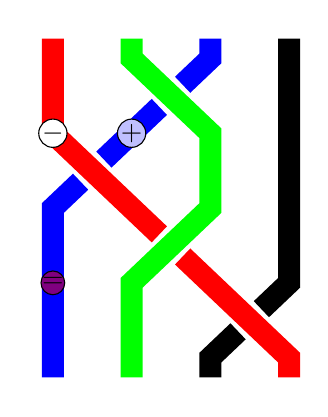
\begin{tikzpicture}
\braid[
  number of strands=3,
  line width=8pt,
  style strands={1}{red},
  style strands={2}{green},
  style strands={3}{blue},
  height=.95cm,
  gap=0.1,
  control factor=0,
  nudge factor=0,
  strand label by origin=false,
  strand label/.style={circle,draw,fill=white,inner sep=0pt},
  yscale=1] (braid_1) a_2 \label[fill=blue!25]{2}{\(+\)} \label{1}{\(-\)} a_1 a_2^{-1} \label[fill=red!50!blue]{1}{\(=\)} a_3;
%\node [at=(braid_1-1-s),circle,draw] {};
\end{tikzpicture}

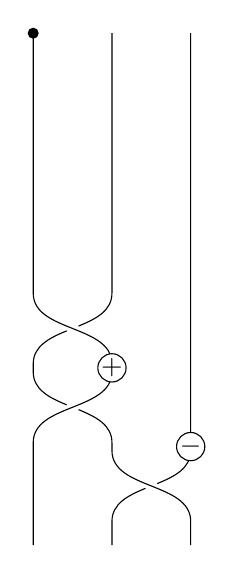
\begin{tikzpicture}
\braid[gap=0.05,strand label/.style={circle,draw,fill=white,inner sep=0pt}] (mybraid) at (3,0) 1 1 1 s_1 \label{2}{\(+\)} s_1^{-1} \label{3}{\(-\)} s_2;
\fill (3,0) circle[radius=2pt];
\end{tikzpicture}
%\end{document}
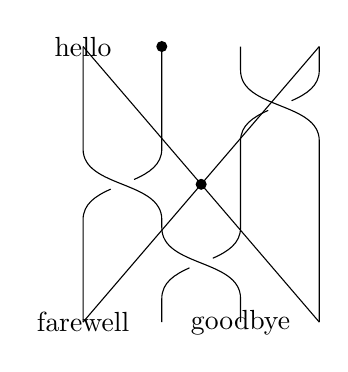
\begin{tikzpicture}
\braid (mybraid) a_3 s_1 s_2;
\node at (mybraid-1-s) {hello};
\node at (mybraid-1-e) {goodbye};
\fill (mybraid-rev-1-s) circle[radius=2pt];
\node at (mybraid-rev-1-e) {farewell};
\fill (mybraid) circle[radius=2pt];
\draw (mybraid-1-s) -- (mybraid-rev-4-e);
\draw (mybraid-4-s) -- (mybraid-rev-1-e);
\end{tikzpicture}


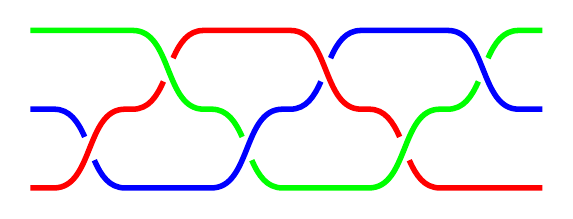
\begin{tikzpicture}
\braid[line width=2pt,style strands={1}{red},style strands={2}{blue},style strands={3}{green},rotate=90] s_1 s_2^{-1} s_1 s_2^{-1} s_1 s_2^{-1};
\end{tikzpicture}

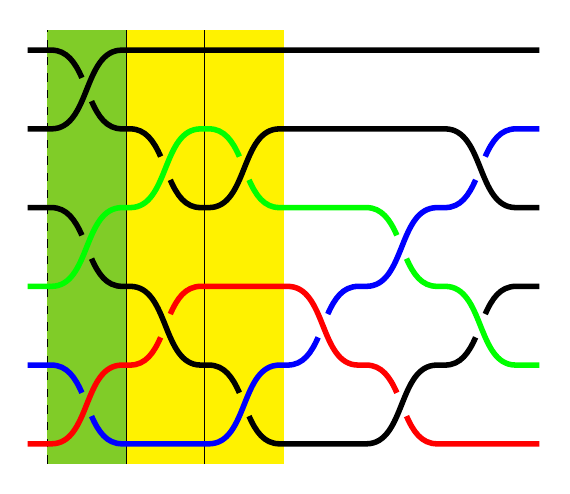
\begin{tikzpicture}
\braid[
  style all floors={fill=yellow},
  style floors={1}{dashed,fill=yellow!50!green},
  floor command={%
    \fill (\floorsx,\floorsy) rectangle (\floorex,\floorey);
    \draw (\floorsx,\floorsy) -- (\floorex,\floorsy);
  },
  line width=2pt,
  style strands={1}{red},
  style strands={2}{blue},
  style strands={3}{green},
  rotate=90
]| s_1-s_3-s_5 | s_2^{-1}-s_4| s_1-s_4 s_2^{-1} s_1-s_3 s_2^{-1}-s_4^{-1};
\end{tikzpicture}
\end{document}


% Local Variables:
% tex-output-type: "pdf18"
% End: